\documentclass{article}
\usepackage[utf8]{inputenc}
\usepackage[english]{babel}
\usepackage[]{amsthm} 
\usepackage[]{amssymb} 
\usepackage{amsmath}
\newcommand{\modwos}[1]{\ (\mathrm{mod}\ #1)}
\usepackage{graphicx}
\usepackage{hyperref}
\usepackage{mathtools}
\usepackage[thinc]{esdiff}
\usepackage[dvipsnames]{xcolor}
\usepackage{float}
\usepackage{listings}
\graphicspath{ {./HW3_img/} }

\title{ADSP: HW3}
\author{Lo Chun, Chou \\ R13922136}
\date\today


\begin{document}
\setlength{\parindent}{0pt}
\maketitle 

\section*{(1)}

In addition to the basic requirements, I also added the following features:
\begin{itemize}
    \item \underline{bpm} (we use the \lstinline{scale_beat_by_bpm} function to scale the beat durations according to the desired BPM)
    \item \underline{octave} (we can use the \lstinline{octave} list to set the octave of each note, so for example, we can have different pitches for "Do" in different octaves)
    \item \underline{rest, note duration} (we can use the \lstinline{beat} list to set the duration of each note, including setting $0$ to present a rest)
\end{itemize}

To check the details of the latter two features, please refer to the \lstinline{getmusic} function in the \lstinline{HW3_1.py} file.

\section*{(2)}

\subsection*{(a)}

By Fermat's little theorem, since $67$ is a prime number, we have:

\begin{align*}
    2^{66} \equiv 1 \modwos{67}
\end{align*}

Then using the fact that:

\begin{align*}
    \text{if } a \equiv b \modwos{n} \text{ then } a^k \equiv b^k \modwos{n} \text{ for any integer } k \in \mathbb{Z}^+
\end{align*}

we have:

\begin{align*}
    &(2^{66})^{10} \equiv 1^{10} \modwos{67} \\
    \Rightarrow \ & 2^{660} \equiv 1 \modwos{67}
\end{align*}

And using the property:

\begin{align*}
    \text{If } a \equiv b \modwos{n} \text{ and } c \equiv d \modwos{n} \text{ then } a \cdot c \equiv b \cdot d \modwos{n}
\end{align*}

We can calculate $2^{40}$:

\begin{align*}
    &2^6 \equiv 64 \equiv -3 \modwos{67} \\
    \Rightarrow \ & (2^6)^6 \equiv (-3)^6 \equiv 243 \times 3 \equiv 42 \times 3 \equiv 126 \equiv -8 \modwos{67} \\
    \Rightarrow \ & 2^{40} \equiv 2^{36} \times 2^4 \equiv (-8) \times 16 \equiv -128 \equiv 6 \modwos{67}
\end{align*}


and combine $2^{40}$ with $2^{660}$, and we'll get the required result:

\begin{align*}
    2^{700} \modwos{67}
    &\equiv 2^{660} \cdot 2^{40} \modwos{67} \\
    &\equiv 1 \cdot 6 \modwos{67} \\
    &\equiv 6 \modwos{67} \qquad \square
\end{align*}

\subsection*{(b)}

We're given the following congruences and are required to find $x \in \mathbb{Z}^+, \quad x \in [0, 2800]$:

\begin{align*}
    x &\equiv 4 \modwos{43} \\
    x &\equiv 15 \modwos{67} 
\end{align*}

Since $\gcd (43, 67) = 1$, we can use the Chinese Remainder Theorem.
\bigskip

Let $n_1 = 43$ and $n_2 = 67$, then we'll have:

\begin{align*}
    &n = n_1 \cdot n_2 = 2881 \\
    &N_1 = \frac{n}{n_1} = 67 \\
    &N_2 = \frac{n}{n_2} = 43 
\end{align*}

And we'll need to solve:

\begin{align*}
    N_1 x_1 \equiv 1 \modwos{n_1} &\implies 67 x_1 \equiv 1 \modwos{43} \\
    N_2 x_2 \equiv 1 \modwos{n_2} &\implies 43 x_2 \equiv 1 \modwos{67}
\end{align*}

Using the Extended Euclidean Algorithm:

\begin{align*}
    67 = 1 \cdot 43 + 24 \quad \Rightarrow &\ 24 = 67 - 1 \cdot 43 \\
    43 = 1 \cdot 24 + 19 \quad \Rightarrow &\ 19 = 43 - 1 \cdot 24 \\
    24 = 1 \cdot 19 + 5 \quad \Rightarrow &\ 5 = 24 - 1 \cdot 19 \\
    19 = 3 \cdot 5 + 4 \quad \Rightarrow &\ 4 = 19 - 3 \cdot 5 \\
    5 = 1 \cdot 4 + 1 \quad \Rightarrow &\ 1 = 5 - 1 \cdot 4
\end{align*}

then we'll get:

\begin{align*}
    1 
    &= 5 - 1 \cdot 4 \\
    &= 5 - 1 \cdot (19 - 3 \cdot 5) \\
    &= 5 - 1 \cdot 19 + 3 \cdot 5 \\
    &= 4 \cdot 5 - 1 \cdot 19 \\
    &= 4 \cdot (24 - 1 \cdot 19) - 1 \cdot 19 \\
    &= 4 \cdot 24 - 5 \cdot 19 \\
    &= 4 \cdot 24 - 5 \cdot (43 - 1 \cdot 24) \\
    &= 9 \cdot 24 - 5 \cdot 43 \\
    &= 9 \cdot (67 - 1 \cdot 43) - 5 \cdot 43 \\
    &= 9 \cdot 67 - 14 \cdot 43
\end{align*}

Thus, $x_1 = 9, \ x_2 = -14 \ (\text{or } x_2 = 53)$.
\bigskip

And the solution $\bar{x}$ is:

\begin{align*}
    \bar{x}
    &\equiv N_1 \cdot x_1 \cdot 4 + N_2 \cdot x_2 \cdot 15 \modwos{n} \\
    &\equiv 67 \cdot 9 \cdot 4 + 43 \cdot (-14) \cdot 15 \modwos{2881} \\
    &\equiv 2412 - 9030 \modwos{2881} \\
    &\equiv -6618 \modwos{2881} \\
    &\equiv 2025 \modwos{2881} \qquad \square
\end{align*}

\subsection*{(c)}

By Wilson's theorem, we knew that if $p$ is a prime, then:

\begin{align*}
    (p-1)! \equiv -1 \modwos{p}
\end{align*}

Thus, since $43$ is a prime, we have:

\begin{align*}
    &42! \equiv -1 \modwos{43} \\
    \Rightarrow \ & 39! \times 40 \times 41 \times 42 \equiv 42 \modwos{43}
\end{align*}

By another property of modular arithmetic, we have:

\begin{align*}
    \text{If } ca \equiv cb \modwos{n} \text{ and } \gcd(c, n) = 1 \text{ then } a \equiv b \modwos{n}
\end{align*}

Therefore, since $\gcd(42, 43) = 1$, we can divide $42$ on both sides:

\begin{align*}
    &39! \times 40 \times 41 \equiv 1 \modwos{43} \\
\end{align*}

Thus, this means that $39!$ is the inverse of $40 \times 41 \modwos{43}$.

\begin{align*}
    40 \times 41 \equiv (-3) \times (-2) \equiv 6 \modwos{43}
\end{align*}


Solving this using the Extended Euclidean Algorithm:

\begin{align*}
    43 = 6 \cdot 7 + 1 \quad \Rightarrow \ 1 = 43 - 6 \cdot 7 
\end{align*}

So we found that the inverse of $6$ is $-7$ or $36 \modwos{43}$. And hence the solution is:

\begin{align*}
    39! \equiv 36 \modwos{43} \qquad \square
\end{align*}


\section*{(3)}

We're given:

\begin{align*}
    M = 11, \ \alpha = 8 + 6i, \ N = 12
\end{align*}

Since we're asked to find CNT of $x$, which is defined as:

\begin{align*}
    F(x)k = \sum_{n=0}^{11} x[n] \cdot \alpha^{kn} \modwos{11} \quad \text{for } k \in \{0, 1, \dots, 11\}
\end{align*}

And we define the CNT matrix $F$ (which is a $12 \times 12$ matrix) as:

\begin{align*}
    F_{k,n} = \alpha^{kn} \modwos{11} \quad \text{for } k, n \in \{0, 1, \dots, 11\}
\end{align*}

Let $p_j = \alpha^j \modwos{11}$ for $j = 0, 1, \dots, 11$, we have:

\begin{align*}
    p_0 &= 1 + 0i \\
    p_1 &= 8 + 6i \\
    p_2 &= 6 + 8i \\
    p_3 &= 0 + 1i \\
    p_4 &= 5 + 8i \\
    p_5 &= 3 + 6i \\
    p_6 &= 10 + 0i \\
    p_7 &= 3 + 5i \\
    p_8 &= 5 + 3i \\
    p_9 &= 0 + 10i \\
    p_{10} &= 6 + 3i \\
    p_{11} &= 8 + 5i \\
\end{align*}

And we can get:

\begin{align*}
    F =
    \begin{bmatrix}
        p_0 & p_0 & p_0 & \cdots & p_0 \\
        p_1 & p_2 & p_3 & \cdots & p_{11} \\
        p_2 & p_4 & p_6 & \cdots & p_{10} \\
        \vdots & \vdots & \vdots & & \vdots \\
        p_{11} & p_{10} & p_9 & \cdots & p_1
    \end{bmatrix}
\end{align*}

From $x$, we can see that:

\begin{align*}
    x[1] = x[5] = x[7] = x[11] = 1, \quad \text{and all other values are zero}
\end{align*}

So:

\begin{align*}
    F(x)_k 
    &= F_{k,1} + F_{k,5} + F_{k,7} + F_{k,11} \\
    &= \alpha^{k \cdot 1} + \alpha^{k \cdot 5} + \alpha^{k \cdot 7} + \alpha^{k \cdot 11} \modwos{11}
\end{align*}

Thus, the resulting vector is:

\begin{align*}
    Fx =
    \begin{bmatrix}
        4 \\
        0 \\
        2 \\
        0 \\
        9 \\
        0 \\
        7 \\
        0 \\
        9 \\
        0 \\
        2 \\
        0
    \end{bmatrix}
    \equiv
    \begin{bmatrix}
        4 \\
        0 \\
        2 \\
        0 \\
        -2 \\
        0 \\
        -4 \\
        0 \\
        -2 \\
        0 \\
        2 \\
        0
    \end{bmatrix}
    \pmod{11} \qquad \square
\end{align*}




\section*{(4)}


Using the following properties:

\begin{align*}
    \left(\frac{2}{p}\right) = 
    \begin{cases}
        1 \quad &p \equiv 1, 7 \modwos{8} \\
        -1 \quad &p \equiv 3, 5 \modwos{8}
    \end{cases}\tag{1}
\end{align*}

And referencing the following table
\footnote{
    \url{https://en.wikipedia.org/wiki/Quadratic_residue}
}:

\begin{figure}[H]
    \centering
    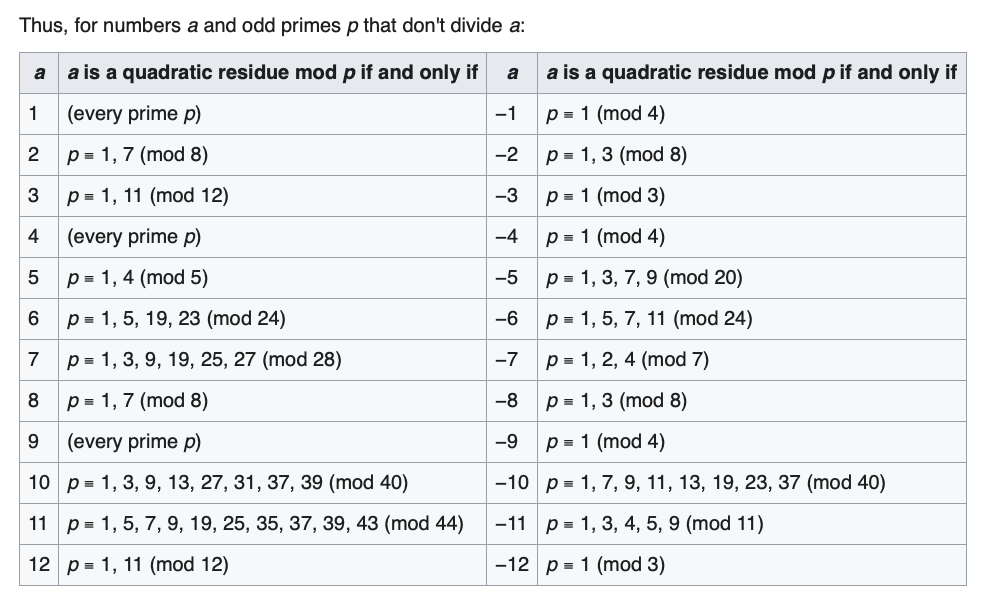
\includegraphics[width=0.8\textwidth]{HW3_img/quadratic_residue.png}
\end{figure}



\begin{align*}
    a \equiv b \modwos{p} \implies \left(\frac{a}{p}\right) = \left(\frac{b}{p}\right) \tag{2}
\end{align*}

\begin{align*}
    \left(\frac{ab}{p}\right) = \left(\frac{a}{p}\right) \left(\frac{b}{p}\right) \tag{3}
\end{align*}

We can calculate the Legendre sequence for $p = 11$:

\begin{align*}
    & \left(\frac{1}{11}\right) = 1 \qquad \because 1 \equiv 1^2 \modwos{11} \\
    & \left(\frac{2}{11}\right) = -1 \qquad \because \text{Using }(1), \ 11 \equiv 3 \modwos{8} \\ 
    & \left(\frac{3}{11}\right) = 1 \qquad \because 3 \equiv 25 \equiv 5^2 \modwos{11} \\
    & \left(\frac{4}{11}\right) = 1 \qquad \because 4 \equiv 81 \equiv 9^2 \modwos{11} \\
    & \left(\frac{5}{11}\right) = 1 \qquad \because 5 \equiv 16 \equiv 4^2 \modwos{11} \\
    & \left(\frac{6}{11}\right) = \left(\frac{2}{11}\right) \left(\frac{3}{11}\right) = (-1) \times 1 = -1 \\
    & \left(\frac{7}{11}\right) = -1 \qquad \text{(Using the table)} \\
    & \left(\frac{8}{11}\right) = \left(\frac{2}{11}\right) \left(\frac{4}{11}\right) = (-1) \times 1 = -1 \\
    & \left(\frac{9}{11}\right) = \left(\frac{3}{11}\right) \left(\frac{3}{11}\right) = 1 \times 1 = 1 \\
    & \left(\frac{10}{11}\right) = \left(\frac{2}{11}\right) \left(\frac{5}{11}\right) = (-1) \times 1 = -1 \\
\end{align*}


Thus, the Legendre sequence for $p = 11$ is:

\begin{align*}
    &\{0, \left(\frac{1}{11}\right), \left(\frac{2}{11}\right), \left(\frac{3}{11}\right), \left(\frac{4}{11}\right), \left(\frac{5}{11}\right), \left(\frac{6}{11}\right), \left(\frac{7}{11}\right), \left(\frac{8}{11}\right), \left(\frac{9}{11}\right), \left(\frac{10}{11}\right)\} \\
    =& \{0, 1, -1, 1, 1, 1, -1, -1, -1, 1, -1\} \qquad \square
\end{align*}

\section*{(5)}

\subsection*{(a)}

We're given:

\begin{align*}
    y[n] = x[n] + 0.4x[n-20] + 0.2x[n-30]
\end{align*}

And need to find $p[n]$ s.t. $y[n] = x[n] * p[n]$
\bigskip

It is trivial that:

\begin{align*}
    p[n] = \delta[n] + 0.4\delta[n-20] + 0.2\delta[n-30] \qquad \square
\end{align*}

\subsection*{(b)}

% From the process in lecture slide p.194, we knew that we can get $P(Z)$ by:

% \begin{align*}
%     P(Z) = 1 + \alpha Z^{-N_p}
% \end{align*}

% Thus, in our case we have:

% \begin{align*}
%     P(Z) = 1 + 0.4Z^{-20} + 0.2Z^{-30}
% \end{align*}

% Taking $\log$ to get $\hat{P}(Z)$:

% \begin{align*}
%     \hat{P}(Z) = \log(1 + 0.4Z^{-20} + 0.2Z^{-30})
% \end{align*}

% Then calculating the inverse Z-transform of $\hat{P}(Z)$:

% \begin{align*}
%     \hat{p}[n] 
%     &= \sum_{k=1}^\infty (-1)^{k+1} \frac{\alpha^k}{k} \delta(n - k \cdot N_p) \\
%     &= \sum_{k=1}^\infty (-1)^{k+1} \frac{0.4^k}{k} \delta(n - 20k) + \sum_{k=1}^\infty (-1)^{k+1} \frac{0.2^k}{k} \delta(n - 30k)
% \end{align*}

The lifter is designed to set to $0$ when $n$ is a multiple of $N_p = 20$ or $30$, 
and set to $1$ otherwise.
\bigskip

Thus, we can design the lifter as:

\begin{align*}
    l[n] = \begin{cases}
        0 & \text{if } n = 20k \text{ or } 30k \text{ for any } k = 1, 2, 3, \cdots \\
        1 & \text{otherwise}
    \end{cases} \qquad \square
\end{align*}


\section*{(6)}

\subsection*{(a)}

It is possible for human to hear voice with freqeuncy $19Hz$.
\bigskip

Even though in theory, the frequency that human can hear is between $20Hz$ and $20000Hz$,
by the lower bound of hearing graph in lecture slide p.238, if the sound intensity ($P$) is high enough,
then it is possible for human to hear.

\subsection*{(b)}

When we're splitting a signal into segments, where each segment present a word, 
we are using the property that consonants have smaller energy than vowels, 
so we can distinguish each word by finding the parts with smaller amplitude.
(This can be seen at p.248 of the lecture note.)
\bigskip

However, for some words with \underline{double vowels}, or there is \underline{no consonant} in the word, 
we can not split the signal by this approach.

\subsection*{(c)}

A music signal always has a the chord phenomenon because music signal is generated by resonance, 
for example, brass instruments generate sound by the vibration of a resonator.
\bigskip

Any sound that is generated by resonance has the effect that at freqeuncy values:

\begin{align*}
    f = k \cdot f_0 \qquad k \in \mathbb{Z}^+
\end{align*}

The amplitude of the signal is larger, which is the chord phenomenon.

\section*{(7)}

\subsection*{(a)}

We can use \underline{entropy} to measure uniformity.

\subsection*{(b)}

The first reason why the compression ratio of an image can be higher than an audio signal because image is of dimension $2D$,
while audio signal is of dimension $1D$, this causes the redundancy of image to be higher than audio signal.
\bigskip

For example, in an image, if there is a pixel of white color, then it is likely that the pixels surrounding it are also white,
and this does not happen only when the pixel is at the edge of an object. This example shows the property of \underline{consistency in space domain}.
\bigskip

Another reason is also due to \underline{consistency} but in the \underline{frequency domain}, 
if we use intensity to represent amplitude, images tend to concentrate on low-frequency components, 
thus, the information that needed to be stored is less.

\subsection*{(c)}

\begin{enumerate}
    \item After transformation and quantization, we can compress symbols by Huffman coding, and this approach is adopted in MP3.
    \item Adaptive Differential Pulse Code Modulation (ADPCM), which uses the fact that neighboring audio samples are often similar to each others (exploit consistency).
    \item MPEG audio compression, which uses masking based on the fact that when there is a strong audio signal, the weaker signal in its neighborhood is more likely imperceptible.
\end{enumerate}

\section*{Extra problem (ID ends with $1, 6$)}

The frequency of a consonant is higher than that of a vowel.

\end{document}